\chapter{Aplica\c c\~oes \textit{mHealth} e arquiteturas relacionadas}



\section{\textit{eHealth}: tecnologias de informação ao serviço da saúde}
Nos dias que correm toda a sociedade tem dispon\'ivel muito facilmente a possibilidade de trocar informa\c c\~ao entre si, podendo permanecer numa constante troca e partilha de informa\c c\~ao.  Com esta realidade tem surgido novas tecnologias, ferramentas e aparelhos que facilitam, tendo em conta a sua implementa\c c\~ao e uso, o fortalecimento da informa\c c\~ao. 
\par
A \'area da sa\'ude cada vez mais est\'a identificada com esta realidade, as tecnologias da informa\c c\~ao e da comunica\c c\~ao t\^em sido um aliado para aumentar a efici\^encia e melhorar a qualidade da presta\c c\~ao de servi\c cos na área da sa\'ude, ajudando a popula\c c\~ao com o seu bem-estar \cite{ict-healthcare}.
\par
Surge então o termo \textit{electronic Health} mais conhecido por \textit{eHealth}, inicialmente utilizado por profissionais de sa\'ude, investigadores e no \^ambito acad\'emico, e est\'a aliado a cen\'arios que envolvem cuidados de sa\'ude, dispositivos eletr\'onicos e a Internet. O termo que at\'e 1999 pouco era utilizado, atualmente \'e um termo que n\~ao define unicamente a ''Medicina na Internet'', mas tamb\'em tudo aquilo que esteja relacionado com computadores e medicina \cite{ehealth}. Podemos ver o \textit{eHealth} como designação abrangente para enquadrar a transformação digital da prestação de cuidados de saúde.
\par A \gls{oms} define \textit{eHealth} \cite{ehealth_oms} como uma ''utiliza\c c\~ao rent\'avel e segura das tecnologias de informa\c c\~ao e comunica\c c\~ao no apoio \`a sa\'ude e \`as \'areas relacionadas com a sa\'ude, incluindo os servi\c cos de sa\'ude, vigil\^ancia na sa\'ude, literatura na sa\'ude, educa\c c\~ao na sa\'ude e investiga\c c\~ao na \'area da sa\'ude.''
\par
Uma defini\c c\~ao apresentada em \cite{ehealth}: ''\textit{eHealth} \'e uma \'area emergente na interce\c c\~ao da inform\'atica m\'edica, sa\'ude p\'ublica e neg\'ocios, referindo-se aos servi\c cos de sa\'ude e entrega de informa\c c\~ao atrav\'es da Internet ou tecnologias semelhantes. Pensando de forma abrangente, o termo n\~ao \'e s\'o um desenvolvimento t\'ecnico, mas tamb\'em uma nova forma de pensar, uma atitude, um compromisso para a rede, um pensamento global, para melhorar o cuidado da sa\'ude local, regional e global com o uso das tecnologias de informa\c c\~ao e comunica\c c\~ao''.
\par
Alguns requisitos tamb\'em s\~ao colocados \cite{ehealth} para um sistema ser considerado \textit{eHealth}, entre eles temos: efici\^encia; melhoria ao n\'ivel de qualidade do cuidado da sa\'ude; sistema baseado em evid\^encias; incentivar uma nova rela\c c\~ao entre o utente e o profissional de sa\'ude; de f\'acil uso.
\par
Temos também a presta\c c\~ao de cuidados de sa\'ude a longa dist\^ancia, mais concretamente a telemedicina. A telemedicina permite a pessoas que estejam localizadas em ambientes mais rurais os cuidados de sa\'ude m\'inimos. A maior parte dos habitantes dos pa\'ises em desenvolvimento moram em zonas rurais dificultando o acesso a servi\c cos de sa\'ude, m\'edicos e tratamentos.\cite{telemedicine-future}
\par
A \gls{oms} define telemedicina como \cite{ehealth_telemedicine} uma ''presta\c c\~ao de cuidados de servi\c cos de sa\'ude em situa\c c\~oes em que a dist\^ancia \'e um fator cr\'itico, por qualquer profissional de sa\'ude usando tecnologias de informa\c c\~ao e comunica\c c\~ao para a partilha de informa\c c\~ao v\'alida para ser feito o diagn\'ostico, o tratamento e a preven\c c\~ao da doen\c ca e danos f\'isicos, pesquisa e avalia\c c\~ao, e para a forma\c c\~ao cont\'inua dos prestadores de cuidados de sa\'ude, com o objetivo da melhoria da sa\'ude dos indiv\'iduos e das suas comunidades''.
\par
A grande vantagem que existe com a utiliza\c c\~ao da telemedicina \'e o custo de deslocamento at\'e uma unidade de sa\'ude e a possibilidade de realiza\c c\~ao de consultas por especialistas de forma remota.
\par
Tendo em conta que a telemedicina e \textit{eHealth}  estão diretamente relacionados, surge ent\~ao a necessidade de existir uma plataforma que possibilite o acesso aos m\'edicos das informa\c c\~oes obtidas dos seus utentes a qualquer momento e em tempo real, estando estes geograficamente em locais distintos.


\section{\textit{mHealth}: computação móvel em saúde}
O termo \textit{\gls{mHealth}} \'e definido segundo a OMS como uma componente da \textit{eHealth} \cite{mhealth_oms} sendo esta definida como, o recurso a dispositivos m\'oveis (como por exemplo o telem\'ovel, \textit{tablet} e outros dispositivos sem fios) para a pr\'atica de cuidados de sa\'ude e m\'edicos.
\par
Uma aplica\c c\~ao \textit{mHealth} pertence tamb\'em \`a componente de \textit{eHealth} assim como \`a telemedicina. As aplica\c c\~oes de \textit{mHealth} t\^em como o objetivo oferecer cuidados de sa\'ude e permitir a m\'edicos a monitoriza\c c\~ao de diferentes par\^ametros desde qualquer lugar e at\'e em movimento, usando dispositivos que fazem parte da componente \textit{eHealth} e transmitindo, esses dados atrav\'es de dispositivos m\'oveis. Como a \textit{mHealth} permite superar as barreiras da localiza\c c\~ao entre os utentes e os m\'edicos podemos dizer que a telemedicina tamb\'em est\'a presente nestas aplica\c c\~oes.
\par
Depois das redes m\'oveis come\c carem a suportar 3G e 4G para transporte de dados, a comunica\c c\~ao m\'ovel tem sido a  principal atra\c c\~ao de investigadores e de comunidades empresariais. Com esta inova\c c\~ao nas redes m\'oveis a presta\c c\~ao de cuidados de sa\'ude em qualquer momento e em qualquer lugar, superando as barreiras geogr\'aficas, temporais e at\'e organizacionais deixou de ser um problema \cite{mhealth}.
\par
As \'areas abrangidas podem ser mesmo bastantes, basta haver aplica\c c\~oes desenvolvidas para o devido efeito e que estejam preparadas para receber dados dos respetivos dispositivos. Este \'ultimo ponto não \'e obrigat\'orio pois os dados podem ser obtidos em dispositivos isoladamente ou adicionados manualmente na aplica\c c\~ao. 
\par
Tomando por exemplo a diabetes, uma doença crónica, há a necessidade de se monitorizar a concentra\c c\~ao de glicose no sangue de doentes com regularidade. Vamos agora analisar um estudo feito nesta área listando algumas aplica\c c\~oes para esta finalidade \cite{mhealth}.

\begin{table}[H]
\centering

\begin{tabularx}{1\textwidth}{|p{3cm}|p{6.1cm}|p{2.7cm}|p{2cm}|}
\rowcolor[HTML]{FFCE93} \hline
\textbf{Aplicação} &  \textbf{Descrição} &  \textbf{Monitorização de parâmetros}  &  \textbf{Leitura Autónoma}  \\
\hline
Daily Carb \cite{mhealth_app1} & Uma aplica\c c\~ao que possibilita uma monitoriza\c c\~ao di\'aria dos nutrientes ingeridos, hidratos de carbono, gorduras e \'agua, assim como leituras da glicose, press\~ao arterial, frequ\^encia card\'iaca, peso, exerc\'icio feito, medica\c c\~ao e insulina ingerida. & Sim & Não \\ \hline

Glucose Buddy \cite{mhealth_app2} & Esta aplica\c c\~ao possibilita aos utilizadores a inser\c c\~ao manual de valores da glicose, hidratos de carbono e insulina ingerida, assim como outras atividades. & Sim & Não \\ \hline
GoMeals \cite{mhealth_app3} & Esta aplica\c c\~ao foi desenvolvida para ajudar o utilizador na escolha de alimentos, atividade e monitoriza\c c\~ao da glicose  para um  estilo de vida saud\'avel. & Sim & Não \\ \hline
\end{tabularx}

\caption{Conjunto de aplicações \textit{mHealth} para ajudar a monitorizar a diabetes}
\label{t:aplications-glicose}
\end{table}

A maioria das aplica\c c\~oes \textit{mHealth} t\^em como foco a capacidade de monitoriza\c c\~ao dos utentes remotamente. Um m\'edico ou um utente pode facilmente aceder aos mesmos dados m\'edicos em qualquer momento e em qualquer lugar atrav\'es de dispositivos m\'oveis como computador, \textit{tablet} ou smartphone. Para isto acontecer é necessário os dados estarem guardados num servidor para serem acedidos tanto pelos médicos como pelos utentes.

Dentro dos dados de saúde mais comuns temos a frequência cardíaca, o \gls{ECG} e o SpO2(Oxímetro de pulso) \cite{wearable-trends}. Estes tipos de dados são os mais comuns, pois são os utilizados quando os doentes estão internados e em avaliação e supervisão contínua.
Dentro destes tipos de dados, considerando agora no caso das aplicações \textit{mHealth} podemos afirmar que o tipo de dados mais comum poderá ser a frequência cardíaca, pois a percentagem de dispositivos eletrónicos que tem este sensor é mesmo enorme. Uma leitura contínua de um \gls{ECG} será também bastante importante para por exemplo a deteção de arritmia.



\newpage
\section{Padrões de arquitetura em aplicações móveis}
Uma aplicação móvel comum é constituída por três camadas principais, entre elas a camada de apresentação que é a camada que compõe a interface com o utilizador da aplicação, a camada de negócio e a camada correspondente aos dados utilizados e guardados pela aplicação. Existe duas perspetivas diferentes ao desenvolver uma aplicação móvel, umas delas é o desenvolvimento de uma aplicação ''rica'' onde a camada de negócio e a camada de dados estão guardadas no próprio dispositivo. A outra perspetiva é o desenvolvimento de uma aplicação ''leve'' onde a camada de negócio e a camada de dados está guardada num servidor. 
\par
No caso de uma aplicação necessitar apenas de um processamento local num cenário ocasional, considera-se desenvolver uma aplicação ''rica'', ou seja, uma aplicação que não tem dependências de qualquer tipo de servidor. Quando uma aplicação tem dependências de servidores considera-se uma aplicação ''leve''. Uma aplicação ''rica'' será uma aplicação mais complexa e difícil de manter pois todas as alterações terão que ser efetuadas ao nível da aplicação.
Na figura \ref{f:mobileapparch} \footnote{Imagem retirada do livro \textit{Mobile Apllications: Architecture, Design, and Development}} podemos ver uma arquitetura comum de uma aplicação móvel. \cite{mobileappbook}

\begin{figure}[H]
  \centering
  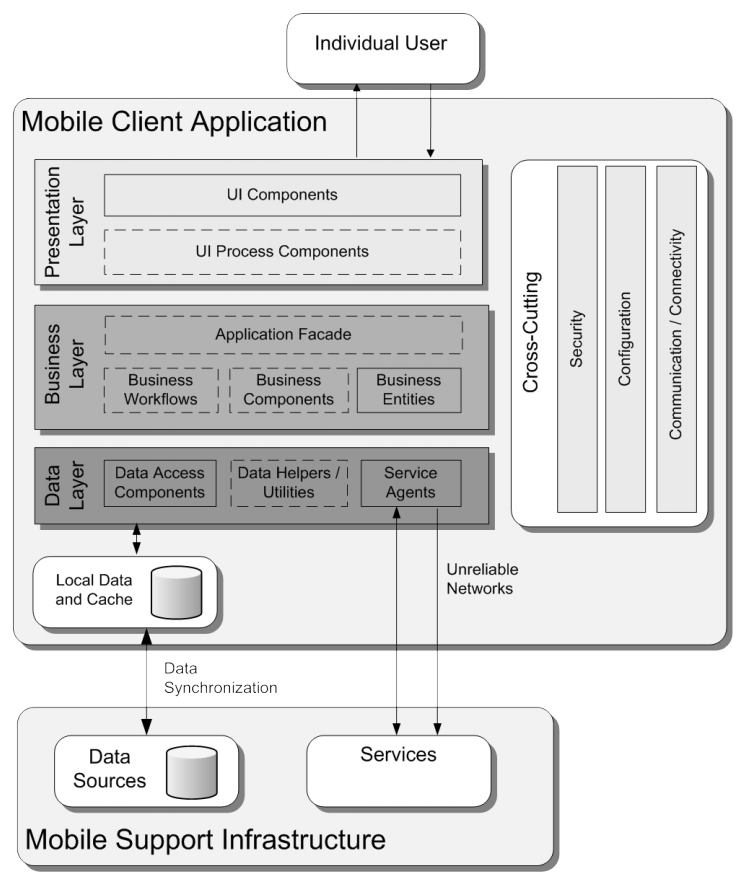
\includegraphics[width=0.6\textwidth]{imgs/mobileapparch.png}
  \caption[Arquitetura t\'ipica de uma  aplica\c c\~ao móvel]{Arquitetura t\'ipica de uma  aplica\c c\~ao móvel. \cite{mobileappbook}}
  
  \label{f:mobileapparch}
\end{figure}

No desenvolvimento de uma aplicação móvel tem que se ter em conta vários fatores importantes para garantir que a aplicação tem os requisitos necessários e é executável em qualquer smartphone. A lista de fatores a ter em conta é bastante alargada mas entre eles temos: Autenticação e Autorização, Armazenamento em \textit{Cache}, Comunicação e Acesso de dados \cite{mobileappbook}. Cada um destes fatores será analisado com mais detalhe de seguida.


\subsection{Autenticação e Autorização}
Uma estratégia de autenticação e autorização eficaz é importante para a segurança e fiabilidade de uma aplicação. Uma fraca autenticação pode deixar a aplicação vulnerável a uma utilização não autorizada. É necessário perceber que existe uma diferença entre autenticação e autorização. A autenticação é o processo de identificação de um utilizador com um identificador único e um elemento secreto (por exemplo uma palavra-passe). Um processo de autenticação garante, após o mesmo, que se trata de um utilizador específico. A autorização é o processo de controlo de ações sobre um serviço. Não indica um utilizador específico por si só. Para isto existe o protocolo de autorização OAuth \cite{oauth20} que é um protocolo padrão para a autorização. Nos dias de hoje grande parte das aplicações utiliza este protocolo de autorização, atualmente vai na versão 2.0 e utiliza \textit{tokens} para ser dada a permissão de acesso a um determinado recurso \cite{oauth20}. De seguida vamos perceber um pouco mais sobre este protocolo de autorização para se perceber a utilidade deste.


\subsubsection{Protocolo de autorização \textit{OAuth}}
O \textit{Open Authorization Protocol} - \textit{OAuth} é um protocolo de autorização que foi desenvolvido com o objetivo de solucionar os problemas relacionados com a gestão de identidades \cite{leiba_oauth}.
\par
Na versão 2.0 do protocolo são definidos quatro pontos de contacto necessários para a compreensão do fluxo de execução deste protocolo, são eles: \textit{Resource Owner} - O proprietário do recurso, que é a entidade que tem o poder de conceder a permissão de acesso, aos seus recursos; \textit{Resource Server} - O servidor de recursos, que é o responsável por guardar e responder às solicitações de acesso aos recursos protegidos, utilizando \textit{tokens} de acesso; \textit{Client} - Cliente, que é uma aplicação, que realiza solicitações de acesso aos recursos protegidos, ao servidor de recursos, em nome do proprietário, dono do recurso, após a obtenção de sua autorização; \textit{Authorization Server} - O servidor de autorização, que é responsável por emitir \textit{tokens} de acesso aos clientes, após autenticar e obter autorização do proprietário dos recursos \cite{oauth20}. Na figura \ref{f:oauth2flow} é apresentado o fluxo do protocolo OAuth 2.0 mostrando a interação entre estes quatro pontos de contacto.

\begin{figure}[H]
  \centering
  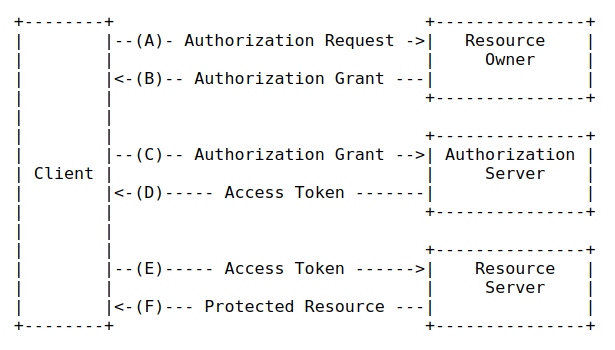
\includegraphics[width=0.8\textwidth]{imgs/oauth2flow.png}
  \caption[Fluxo do Protocolo 2.0]{Fluxo do Protocolo de autorização OAuth 2.0. \cite{oauth20}}
  \label{f:oauth2flow}
\end{figure}

\begin{enumerate}[label=(\Alph*)]
    \item O \textit{Client} pede autorização ao \textit{Resource Owner} para aceder aos seus recursos.
    \item Assumindo que o \textit{Resource Owner} autoriza o acesso, o \textit{Client} recebe um \textit{authorization grant} (garantia de autorização). Essa credencial representa a autorização concedida pelo \textit{Resource Owner}.
    \item O \textit{Client} pede um \textit{token} de acesso ao \textit{Authorization Server}, enviando o \textit{authorization grant}.
    \item Assumindo que o \textit{Client} foi autorizado com sucesso e que o \textit{authorization grant} é válido, o \textit{Authorization Server} gera um \textit{token} de acesso, sendo este enviado para o \textit{Client}.
    \item O \textit{Client} pede acesso a um recurso protegido pelo \textit{Resource Server}, e autentica-se utilizando o \textit{token} de acesso.
    \item Assumindo que o \textit{token} de acesso é válido, o \textit{Resource Server} responde ao pedido do \textit{Client} enviando o recurso pedido.
\end{enumerate}


\subsection{Armazenamento em \textit{Cache}}
A utilização da \textit{cache} do dispositivo pode ser muito importante para aumentar o desempenho e a capacidade de resposta de uma aplicação. Quando não existe ligação à internet, a aplicação deve suportar a execução das operações principais, isto é, se uma aplicação tem como objetivo obter a frequência cardíaca de um paciente, é suposto se conseguir obter estes dados dos sensores mesmo sem estes poderem ser guardados no servidor, ou seja, podem ser guardados em \textit{cache} até que se tenha possibilidade de fazer o envio para o servidor.\par
Recentemente a Google fez recomendações para a utilização de uma componente da arquitetura do Android denominada por Biblioteca de Persistência \cite{cache-android} que é utilizada para a criação de repositórios locais no sentido de \textit{cache}, tornando as aplicações mais resilientes à variabilidade da qualidade do serviço de uma rede.


\subsection{Comunicações}
Os dispositivos móveis comunicam essencialmente com tecnologia sem fios. A comunicação com servidores decorre habitualmente sobre IP. Na transmissão entre servidores temos que ter em conta que temos que proteger os dados que estarão a ser transportados contra roubo ou adulteração. Para comunicação entre dispositivos móveis é utilizada a tecnologia \textit{bluetooth}.


\subsubsection{\textit{Bluetooth}}
O \textit{bluetooth} é uma tecnologia que foi criada em 1994, como uma alternativa sem fios para cabos de dados através da utilização de transmissões de rádio para ligar os dispositivos relativamente próximos, e transferir dados entre eles. Esta tecnologia foi criada como um padrão aberto para permitir a conectividade e a colaboração entre diferentes produtos e indústrias \cite{bluetooth}.
Esta tecnologia está presente em grande percentagem de dispositivos eletrónicos vendidos atualmente, e quase todos os \textit{smartphones} têm esta tecnologia.
\par 
Para a comunicação entre os sensores e os dispositivos móveis ser estabelecida ambos têm que ter pelo menos uma interface de comunicação em comum, isto é, um sensor \textit{bluetooth} tem um conjunto de perfis \textit{bluetooth} a partir do qual os dispositivos móveis podem se conectar e estabelecer uma ligação recolhendo os dados. 
Os perfis disponibilizam padrões que devem ser respeitados para permitir que dispositivos utilizem o \textit{bluetooth} de uma maneira normalizada. \cite{bluetooth-article}
\par
Um dos perfis é denominado de \textit{\gls{HDP}}, foi um perfil criado com o objetivo de se normalizar a comunicação entre dispositivos e sensores na área da saúde utilizando a tecnologia \textit{bluetooth}. Os mesmo dados pode ser enviados utilizando um perfil mais comum, este perfil é o \textit{\gls{SPP}} mas não está configurado para a comunicação de dispositivos na área da saúde \cite{bt-article}.

\subsection{Tecnologias para a implementação de serviços}
Vamos agora rever tecnologias com interesse direto para a implementação e adaptação da plataforma que vai ser apresentada mais à frente.
\subsubsection{\textit{Web Services}}
Os \textit{Web Services} ou serviços \textit{web} permitem que duas máquinas diferentes comuniquem entre si, ou que dois pedaços de código comuniquem entre eles. Para isto funcionar tem que existir um servidor que disponibilize uma \textit{\gls{API}} que é um conjunto de métodos, e então os clientes podem chamar esses métodos e comunicar com o servidor pela Internet por serviços \textit{web}. Uma vantagem da utilização dos serviços \textit{web} é que atualmente é uma tecnologia padrão, ou seja, é uma tecnologia que não é especifica de nenhuma linguagem de programação. Podem estar os serviços \textit{web} desenvolvidos em Java, e os pedidos podem ser efetuados através de um cliente que está a correr em Python. O único formato de dados utilizado por um serviço \textit{web} era o \textit{\gls{XML}}, e só apenas mais tarde começou a poder ser utilizado o \textit{\gls{HTML}} e o \gls{JSON} depois do aparecimento do \textit{\gls{REST}} \cite{wsjakob}.



\subsubsection{ REST \textit{Web Services}}
O \gls{REST} é um estilo de arquitetura que utiliza o \textit{\gls{HTTP}} para fazer chamadas entre máquinas e tem como objetivo fundamental facultar serviços para ajudar no desenvolvimento de aplicações \cite{whatisrest}.
\gls{REST} caracteriza uma arquitetura centrada em recursos, especificando que cada recurso é identificado por um \textit{\gls{URI}}, mediante o qual um conjunto de operações pode ser aplicado através de uma interface uniforme. Esta interface padrão uniforme para a comunicação entre servidores e clientes é o \gls{HTTP} e, em vez de declarar métodos, são aplicadas ações \gls{HTTP}, tais como POST, GET, PUT e DELETE. Estas quatro ações podem ser mapeadas para as ações típicas de dados \textit{\gls{CRUD}}. A representação de cada recurso identificado por um URI, pode variar, podendo ser representado em \gls{XML}, \gls{HTML}, \gls{JSON}, entre muitas outras possibilidades \cite{restwebservices}.



\subsubsection{Vert.x}
É uma \textit{framework} orientada a eventos e assíncrona, que permite a criação de aplicações facilmente escaláveis de uma forma simples, pode ser utilizada por pequenas aplicações, por aplicações \textit{web} sofisticadas e modernas e ainda para o desenvolvimento de micro serviços \gls{HTTP}/\gls{REST}\cite{vertx-io}.
O Vert.x é uma \textit{framework} poliglota, ou seja, tem suporte para várias linguagens de programação, orientada a eventos, construída segundo o padrão reativo e assente na \textit{\gls{JVM}}. 
O Vert.x é composto por um conjunto de componentes que são importantes para o desenvolvimento de aplicações. Entre eles temos: 
\begin{itemize}
  \item \textit{Verticle}: Um \textit{verticle} é definido por ter uma função principal (\textit{main}), que corre um \textit{script} específico. Um \textit{verticle} pode ser escrito em múltiplas linguagens (Java, Javacript, Ruby, Groovy, Ceylon, Scala e Kotlin). Vários \textit{verticles} podem ser executados na mesma instância do Vert.x.
  \item \textit{EventLoops}: São \textit{threads} que estão sempre a correr e estão sempre à escuta, de forma a verificar se existem operações a executar ou dados a tratar. A gestão destas \textit{threads} é feita por uma instância do Vert.x, que aloca um número específico de \textit{threads} a cada núcleo do servidor.
  \item \textit{Handler}: É uma entidade que recebe mensagens do \textit{eventbus} depois de se registar num determinado endereço.
  \item \textit{EventBus}: Esta é uma característica do Vert.x bastante importante que permite a comunicação entre vários \textit{verticles}. Para além disso, é possível haver uma comunicação não só entre \textit{verticles} mas entre entidades que registem \textit{handlers} num servidor (ex. clientes). Desta forma é possível a entrega das mensagens a todos os \textit{handlers} que estiverem registados num determinado endereço. Esta característica é um padrão na troca de mensagens conhecido por \textit{publish–subscribe}.
\end{itemize}
Na figura \ref{f:vertxarch} podemos visualizar uma arquitetura simples do Vert.x. \cite{vertx-study}

\begin{figure}[H]
  \centering
  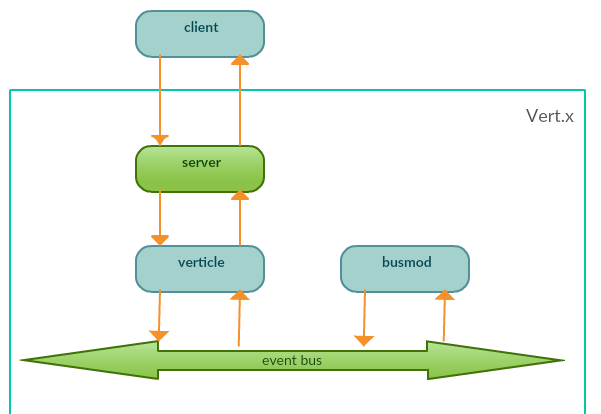
\includegraphics[width=0.6\textwidth]{imgs/vertx_arch.png}
  \caption[Arquitetura simples do Vert.x]{Arquitetura simples do Vert.x (Adaptado de: \cite{vertx-study})}
  \label{f:vertxarch}
\end{figure}


\subsubsection{JSON}
O \gls{JSON} é um formato de dados baseado em texto, é compacto e utilizado para troca de informação independentemente da linguagem a ser utilizada. O \gls{JSON} é baseado em pares atributo-valor e a sua sintaxe é composta por quatro tipos de dados primitivos (\textit{strings}, inteiros, \textit{booleans} e \textit{null}) e dois tipos estruturados (objetos e vetores) \cite{json}. 
\par
É um formato de dados  fácil de gerar, compreender e interpretar. Analisando um documento \gls{JSON} é intuitivo associar a sua aparência, estrutura e sintaxe a muitas linguagens de programação existentes, razão pela qual foi facilmente adotada como uma alternativa ao \gls{XML} por parte de diversos programadores que viram no novo formato um modo mais natural e simples de definir dados.



\newpage
\section{O \textit{backend} nas aplicações de \textit{mHealth}}
O termo \textit{backend} é utilizado para agrupar tudo aquilo que é executado no lado do servidor e que dá suporte a uma aplicação. Tipicamente a arquitetura das aplica\c c\~oes mHealth utiliza a Internet e serviços \textit{web} para disponibilizar uma intera\c c\~ao entre os utentes e os m\'edicos \cite{mhealth}. Podemos ver na figura \ref{f:mhealtharch} que do lado do utente temos a aplicação móvel que permite ligar-se a sensores ou dispositivos especializados para fazer a colheita de novos dados fisiológicos e posteriormente fazer o envio para o servidor através de um serviço \textit{web}. Do lado do servidor podemos ter sistemas de monitorização remotos que podem entrar em contacto com o utente ou médico em situações de emergência.

\begin{figure}[H]
  \centering
  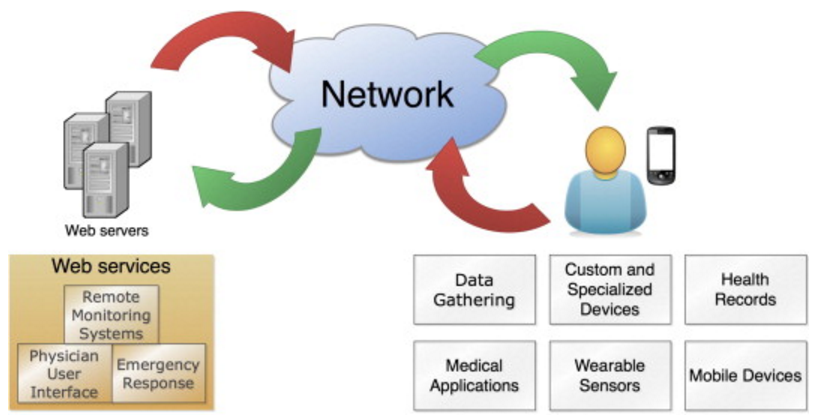
\includegraphics[width=0.7\textwidth]{imgs/mHealthArch.png}
  \caption[Arquitetura t\'ipica de uma  aplica\c c\~ao \textit{mHealth}]{Arquitetura t\'ipica de uma  aplica\c c\~ao \textit{mHealth}. \cite{mhealth}}
  
  \label{f:mhealtharch}
\end{figure}



\subsection{O \textit{backend} no desenvolvimento de uma aplica\c c\~ao \textit{mHealth}}
As solu\c c\~oes de \textit{mHealth} que abrangem estes seis princ\'ipios t\^em uma maior probabilidade de sucesso: Interoperabilidade, Integra\c c\~ao, Intelig\^encia, Socializa\c c\~ao, Resultados e Compromisso \cite{mhealthinsights}. Seguindo estes princípios as aplicações desenvolvidas terão a capacidade de ser interoperáveis com diferentes dispositivos móveis e terão a capacidade de importar e exportar registos de saúde eletrónicos com e para outras aplicações. Terá também a capacidade de ser integrada em algumas atividades físicas dos pacientes e de analisar os dados fornecendo uma monitorização em tempo real. Será também importante a partilha dos dados em redes sociais e em plataformas de saúde para receber apoio e algumas recomendações. A aplicação terá também que ter a capacidade de se adaptar à utilização dos pacientes tendo em conta os dados recolhidos pelos utentes para posteriormente preparar a aplicação para um melhor apoio e monitorização\cite{mhealthinsights}.
\par
Apesar das aplica\c c\~oes \textit{mHealth} estarem numa crescente popularidade nos \'ultimos anos, muitas delas s\~ao rejeitadas ou n\~ao utilizadas pelo p\'ublico alvo pretendido. Para analisar esta realidade foi feito um estudo para se saber os requisitos e as considera\c c\~oes a ter durante e antes do desenvolvimento de uma aplica\c c\~ao \textit{mHealth}\cite{mhealth-pipeline}.
\par
Depois deste estudo e discuss\~ao chegaram \`a conclus\~ao que o desenvolvimento de uma aplica\c c\~ao deve estar dividida em 4 partes distintas criando uma pipeline de desenvolvimento, entre elas temos:  Prepara\c c\~ao, Desenvolvimento do \textit{Back-End}, Desenvolvimento do \textit{Front-End} e Lan\c camento da Aplica\c c\~ao\cite{mhealth-pipeline}. \par 
A secção de Preparação descreve as etapas que estão envolvidas na preparação da aplicação, identificando o problema que vai ser resolvido, uma proposta de solução e o público alvo. É constituída por várias subsecções, entre elas temos: Propósito, Tipo de aplicação e Ética/ Regulamentos \cite{mhealth-pipeline}. 
\par 
Relativamente ao Desenvolvimento do \textit{Back-End} tem que se ter em consideração que vamos estar a lidar com dados e informações sensíveis e pessoais relacionados com o utente. Por isto deve se ter em atenção o envio, registo e armazenamento dos dados e informações no servidor. Para isso temos que ter em atenção algumas questões relacionadas com a segurança e privacidade dos dados \cite{mhealth-pipeline}.
\par 
A secção Desenvolvimento do \textit{Front-End} serve para se decidir o desenvolvimento da aplicação. Para isso deverá-se ter em conta o público alvo, desenvolvendo um ambiente com uma boa experiência de utilização satisfazendo ao máximo, os especialistas e os utentes envolvidos. Um dos requisitos da interface de utilizador deverá ser direcionada para as necessidades do utente e do especialista. Existe também cuidados a ter em conta, mas isso depende da aplicação tendo em conta a sua finalidade e considerações. Nestas considerações podemos incluir que a aplicação pode vir a ser utilizada por pessoas  cegas, surdas, pessoas com mobilidade limitada ou dificuldades de aprendizagem, contexto social, contexto cultural e idade \cite{mhealth-pipeline}.
\par 
A secção do Lançamento da aplicação descreve o processo de conclusão e lançamento da aplicação. Daqui para a frente pode ser necessário consultar ajuda externa de pessoas especialistas em \textit{marketing} \cite{mhealth-pipeline}. 




\subsection{A escolha de um \textit{backend}}
Para dar suporte à aplicação móvel é necessário a escolha de um \textit{backend} robusto e seguro para que possamos lidar com dados e informações sensíveis e pessoais relacionados com o utente. Por isto deve ter-se em atenção o envio, registo e armazenamento dos dados e informações no servidor. Para isso temos que ter em atenção algumas questões relacionadas com a segurança e privacidade dos dados. A escolha de um \textit{backend} para dar suporte às aplicações \textit{mHealth} é bastante importante. Ao utilizar uma plataforma já desenvolvida e reconhecida estamos a aumentar as funcionalidades da aplicação pois estamos a permitir uma futura interoperabilidade e troca de dados entre outras aplicações que utilizem a mesma plataforma.




\subsubsection{\textit{Open mHealth}}
A \textit{\gls{OMH}} foi fundada em 2011 e descreve-se a si própria como "uma \textit{start-up} sem fins lucrativos que quebra as barreiras de integração trazendo significado aos dados clínicos digitais na área da saúde" \cite{omhabout}. A \gls{OMH} trabalha com especialistas da área da saúde e com programadores com o objetivo de tornar os dados de saúde digitais úteis e possíveis de utilizar em diversas plataformas. \par 
Um dos principais objetivos desta organização é que as aplicações na área da saúde não utilizem cada uma delas um formato de dados fechado e próprio, pois desta maneira os dados só são úteis dentro da própria aplicação, ou seja, estes não podem ser exportados para bases de dados de hospitais, ou clínicas, ou ainda outras aplicações na área da saúde. Podemos ver na figura \ref{f:omharch} a diferença que existe entre cada aplicação utilizar um formato de dados próprio, ou utilizar todas o mesmo formato\cite{omharticle}. Do lado esquerdo podemos verificar que existe desenvolvimentos diferentes para cada aplicação, enquanto que utilizando o \gls{OMH} todas podem utilizar a mesma maneira de guardar os dados, ou até, utilizar o mesmo servidor para guardar os dados.
\begin{figure}[H]
  \centering
  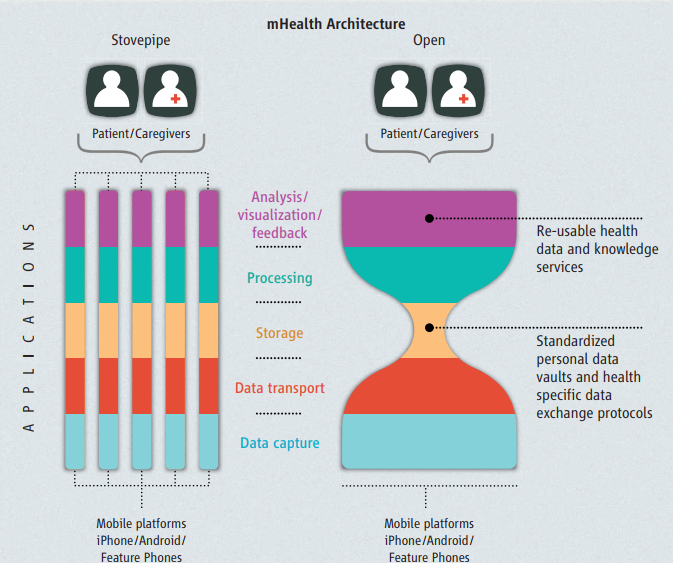
\includegraphics[width=0.8\textwidth]{imgs/openmharch.png}
  \caption[Arquitetura mHealth: Própria vs \textit{Open}]{Arquitetura mHealth: Própria(''afunilada'') vs \textit{Open}. \cite{omharticle} A utilização de uma plataforma aberta reduz o esforço e o desenvolvimento nas tarefas de gestão dos dados}
  
  \label{f:omharch}
\end{figure}

Através desta arquitetura podem ser partilhados diversos recursos entre as aplicações móveis na área da saúde, entre eles o mais importante é o modo e o local onde os dados são guardados, respeitando um padrão para o formato dos dados, ou seja, se duas aplicações diferentes forem guardar dados de um determinado tipo, como por exemplo frequência cardíaca, esses dados têm que respeitar um determinado formato, sendo estes guardados da mesma maneira independentemente da aplicação que o esteja a fazer.
\par 
A \gls{OMH} tem definido um conjunto de \textit{data schemas} que é um conjunto de esquemas de dados (\textit{schemas}) criados e disponíveis que especificam um formato de dados para um determinado conteúdo como por exemplo a frequência cardíaca\cite{omhschemas}. Estes \textit{data schemas} estão desenvolvidos em \gls{JSON} \textit{schema} que serve para descrever um formato de dados, e os programadores têm que ter o cuidado de os dados inseridos e criados sejam  compatíveis com o \gls{JSON} \textit{schema} associado. Na figura \ref{f:exemplo} podemos ver um exemplo de dados que é compatível com o \gls{JSON} \textit{schema} da figura \ref{f:hrjsonschema} associado que é a frequência cardíaca\cite{omhheartrate}.
\newpage

\begin{figure}[H]
\inputminted[fontsize=\scriptsize]{json}{code/hr-jsonschema.json}
\caption[\gls{JSON} \textit{schema} que define o tipo de dados para a frequência cardíaca]{\gls{JSON} \textit{schema} que define o tipo de dados para a frequência cardíaca \cite{omhheartrate}}
\label{f:hrjsonschema}
\end{figure}

\begin{figure}[H]
\inputminted[fontsize=\scriptsize]{json}{code/heart-rate.json}
\caption[Exemplo de um \gls{JSON} compatível associado à frequência cardíaca]{Exemplo de um \gls{JSON} compatível associado à frequência cardíaca \cite{omhheartrate}}
\label{f:exemplo}
\end{figure}
Existe uma implementação de uma \textit{\gls{REST}full \gls{API}} denominada por \textit{dataPoint API} que suporta a criação, consulta e eliminação de dados inseridos. Esta \gls{API} permite a autorização utilizando o protocolo de autorização OAuth 2.0. Um \textit{dataPoint} é um documento \gls{JSON} composto por um cabeçalho e um \textit{body}, em que o \textit{body} representa um tipo de dados e está em conformidade com o \textit{dataschema} definido no cabeçalho.



\subsubsection{FHIR}
Como vimos anteriormente para que os sistemas de serviços hospitalares comuniquem e partilhem  informação entre si, e com as plataformas online, é imperativo que compreendam o que está a ser comunicado.
\par 
Para compreenderem o que está a ser comunicado, os sistemas hospitalares e plataformas devem acordar na norma de comunicação. Existem várias normas para a troca de informação clínica. Existe uma norma que é o \textit{\gls{HL7}} que é tipicamente utilizada em sistemas hospitalares \cite{whyihe} e tem ganho popularidade na troca de informação clínica estruturada.
A organização que definiu o \gls{HL7} desenvolveu a sua própria \gls{API} e formatos de dados denominada de \textit{\gls{FHIR}} \cite{hl7fhir}. O \gls{FHIR} consiste numa definição de uma \gls{API} e conjunto de dados normalizados com o objetivo de fornecer mecanismos de interoperabilidade para o \gls{HL7}, baseados nas tecnologias existentes na web, tais como \gls{XML}, \gls{JSON} , \gls{HTTP}, OAuth, entre outros \cite{hl7fhir}. Este suporta arquiteturas baseadas em \gls{REST} e é suficientemente flexível para ser utilizado em diversos contextos, tais como aplicações móveis ou partilha de registos clínicos eletrónicos \cite{hl7fhir}.

\textbf{HL7}
\par
A norma HL7 é utilizada para troca, integração, partilha e requisição de  registos clínicos em formato eletrónico\cite{hl7}.
O HL7 encontra-se atualmente na sua versão 3\cite{corepointhealth}, mas a versão 2 do \gls{HL7} ainda é bastante utilizada, especialmente em sistemas antigos. 
\par
O problema que existia na versão 2 do \gls{HL7} é que cada sistema hospitalar ou clínica podia adaptar a norma à sua medida. Como esta versão 2 não possui um modelo explícito de informação(mas definições vagas para muitos campos de dados) e também campos opcionais. Estas características conferem-lhe uma maior flexibilidade, mas tornam necessários acordos bilaterais detalhados de forma a permitir a interoperabilidade entre os sistemas envolvidos. Quando estes acordos não são efetuados, se formos desenvolver uma aplicação que comunica com vários sistemas hospitalares ou clínicos, é necessário implementar uma interface especifica para cada um deles.
\par
Para resolver este problema saiu a versão 3, mas a sua adoção não é ainda generalizada \cite{corepointhealth}.
A versão 3 do HL7 foi desenvolvida com base num modelo de dados orientado a objetos, denominado por \textit{Reference Information Model (\gls{RIM})}. Este é constituído por 4 classes principais, tendo como objetivo garantir a interoperabilidade semântica que não existia nas versões anteriores. Estas quatro classes principais são: Entidade, Papel/Cargo, Participação e Ato\cite{hl7-rim}.
\par 
O modelo \gls{RIM} é construído à volta de 5 conceitos principais:
\begin{itemize}
  \item Todo o acontecimento é um ato
  \item Atos estão relacionados com um participante
  \item A participação define o contexto de um ato
  \item Os participantes têm um papel/cargo
  \item Cada cargo/papel é desempenhado por uma entidade
\end{itemize}

Na figura \ref{f:rimclass} podemos visualizar a class \gls{RIM} da versão 3 do HL7.

\begin{figure}[H]
  \centering
  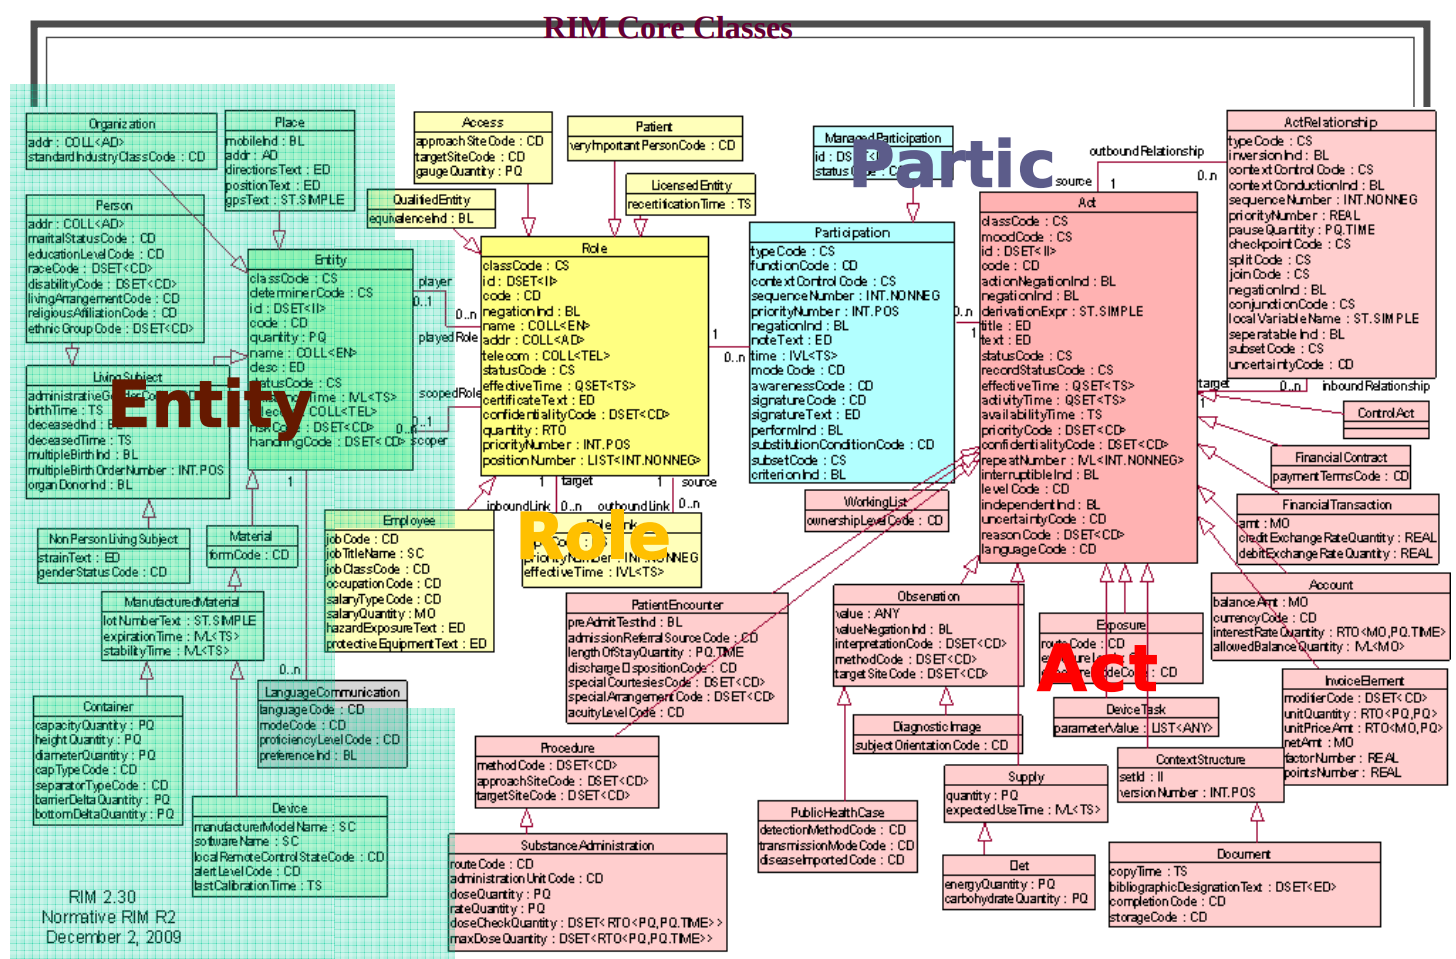
\includegraphics[width=0.9\textwidth]{imgs/hl7-rim.png}
  \caption[Classes principais do \gls{RIM}]{Classes principais do \gls{RIM} \cite{hl7-rim}}
  
  \label{f:rimclass}
\end{figure}




\subsubsection{\textit{Google Fit}}
O \textit{Google Fit} é uma \gls{API} \gls{REST} desenvolvido pela Google, na área do \textit{fitness}. Permite aos utilizadores armazenar e aceder a informação relativa à sua condição física. Apesar de não ter sido desenvolvido com o objetivo de controlar os dados de saúde dos pacientes, pode ser visto como uma plataforma que cumpre alguns desses objetivos.
\par 
O \textit{Google Fit} é mais utilizado com o objetivo de monitorizar a condição física dos seus utilizadores, mas a Google permite o acesso aos dados recolhidos, através de \gls{API}’s criadas para esse efeito. Isto permite a criação de aplicações de saúde, visto que também é um dos objetivos da Google a integração de qualquer aparelho sensor. Resumindo, são dadas todas as ferramentas necessárias ao programador para aumentar o alcance da plataforma, permitindo-a ser utilizada com finalidades que a Google neste momento não cobre. 
Na figura \ref{f:googleFitOverview} mostramos uma vista geral da plataforma \textit{Google Fit}.

\begin{figure}[!ht]
  \centering
  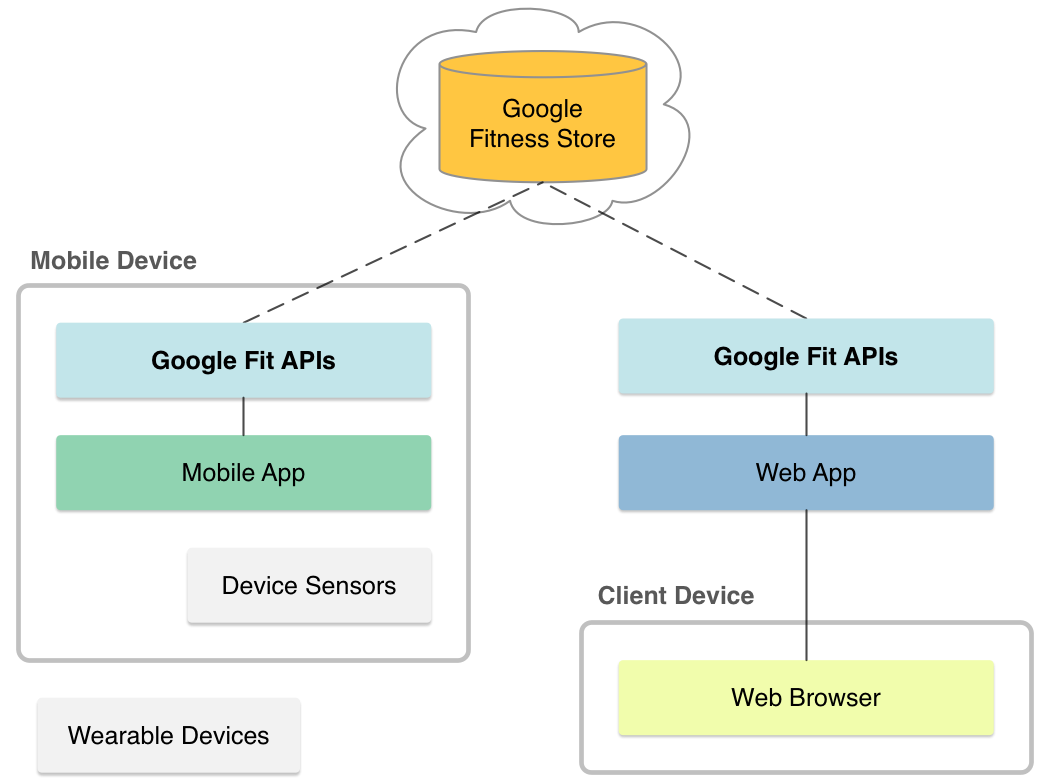
\includegraphics[width=0.7\textwidth]{imgs/googleFitOverview.png}
  \caption[Vista geral da plataforma \textit{Google Fit}]{Vista geral da plataforma \textit{Google Fit} \cite{googlefit}}
  
  \label{f:googleFitOverview}
\end{figure}

Como podemos perceber, existem duas possibilidades diferentes de interagir com a plataforma. Através de uma aplicação para \textit{smartphones} com o sistema operativo \textit{Android}, desenvolvida também pela Google.  Também é possível a utilização de um \textit{website}, que será um pouco mais limitado, mas se for apenas para visualizar os dados já inseridos na plataforma é bastante viável.

A \gls{API} \gls{REST} dá flexibilidade ao sistema. Com a utilização da \gls{API} passa a ser possível a criação de aplicações para outras plataformas que não o \textit{Android}, tornando o \textit{Google Fit} apelativo para um maior número de utilizadores. Esta \gls{API} está protegida pelo protocolo de autorização OAuth 2.0 e utiliza para formato dos dados \gls{JSON}\cite{googlegetstarted}. 



\subsubsection{Análise Comparativa}
Foi ainda feito um breve estudo em relação a outros três possíveis \textit{backends}, entre eles temos o \textit{Health Vault} \footnote{https://international.healthvault.com}, \textit{Apple Research Kit} \footnote{https://www.apple.com/pt/researchkit/} e o \textit{Research Stack} \footnote{http://researchstack.org/}. O estudo não foi tão aprofundado como os apresentados anteriormente mas ainda assim serve para análise comparativa na tabela \ref{t:analisecomparativa} \footnote{ - - nenhum suporte; - suporte fraco; + suporte suficiente; ++ muito bem suportado; n/a não aplicável}. Os requisitos analisados relativamente a cada possível \textit{backend} foram: 
\begin{itemize}
  \item Possibilidade de guardar dados demográficos dos utentes.
  \item Análise do grau de complexidade  do \textit{backend} para adaptação e implementação de novas funcionalidades.
  \item Estruturas de dados normalizadas para uma possível importação/exportação dados de/para outros \textit{backends}.
  \item Possibilidade de adicionar novas estruturas de dados .
  \item Questões relativas a Segurança e Privacidade sobre os dados recolhidos e demográficos.
  \item Capacidade de ser integrado em ambientes diferentes, como android, ios ou web.
  \item Código Aberto quanto à própria implementação do \textit{backend}.
\end{itemize}

\begin{table}[H]
\centering

\label{tabelaComparativa}
\begin{tabular}{|>{\columncolor[HTML]{C0C0C0}}c |c|c|c|c|c|c|}
\hline
\textbf{\backslashbox{Requisito}{Plataforma}}                                                                        & \cellcolor[HTML]{C0C0C0}\textbf{OMH} & \cellcolor[HTML]{C0C0C0}\textbf{FHIR} & \cellcolor[HTML]{C0C0C0}\textbf{\begin{tabular}[c]{@{}c@{}}\textit{Google}\\ \textit{Fit}\end{tabular}} & \cellcolor[HTML]{C0C0C0}\textbf{\begin{tabular}[c]{@{}c@{}}\textit{Health}\\ \textit{Vault}\end{tabular}} & \cellcolor[HTML]{C0C0C0}\textbf{\begin{tabular}[c]{@{}c@{}}\textit{Apple}\\ \textit{Research}\\ \textit{Kit}\end{tabular}} & \cellcolor[HTML]{C0C0C0}\textbf{\begin{tabular}[c]{@{}c@{}} \textit{Research}\\ \textit{Stack}\end{tabular}}  \\ \hline

\textbf{Dados do Paciente} & - & + + & - & + + & + + & + + \\ \hline

\textbf{\begin{tabular}[c]{@{}c@{}}Facilidade de \\ Desenvolvimento\end{tabular}} & + + & + & + + & - & n/a & n/a \\ \hline

\textbf{\begin{tabular}[c]{@{}c@{}}Modelo de Dados \\ Normalizado\end{tabular}} & + & + + & - - & - - & n/a & n/a \\ \hline

\textbf{\begin{tabular}[c]{@{}c@{}}Extensibilidade do \\ Modelo de Dados\end{tabular}} & + + & + & + & + & n/a & n/a \\ \hline

\textbf{Segurança e Privacidade} & + + & + + & + + & + + & + + & + + \\ \hline

\textbf{MultiPlataforma} & + + & + + & + + & + + & n/a & n/a \\ \hline

\textbf{Código Aberto} & + + & + & - & - & n/a & n/a \\ \hline

\end{tabular}
\caption{Comparação dos diferentes \textit{backends}}
\label{t:analisecomparativa}
\end{table}

Depois de analisados seis serviços de \textit{backend} para dar suporte a uma aplicação móvel na área de saúde, faz-se aqui uma breve análise comparativa das suas características. Cada um apresenta vantagens nuns aspetos e desvantagens noutros.
\par 
A grau de complexidade do \gls{FHIR} é bastante elevado devido à sua grande dimensão. É um \textit{backend} bastante completo apesar da extensibilidade dos tipos de dados não ser trivial. Relativamente aos tipos de dados a ser guardados falta contemplar o \gls{ECG} e o acelerómetro \footnote{Estes dados fazem parte do conjunto de dados a ser guardado no sistema mais à frente, neste momento serve também para avaliar a capacidade da cada plataforma para os suportar/integrar}, pois estes não estão contemplados.
\par 
Em relação ao \textit{Google Fit} tem uma boa \gls{API} \gls{REST}, apesar de não haver nenhum tipo dados onde se pudesse guardar os dados do paciente e o \gls{ECG}. A extensibilidade do modelo de dados é possível mas existe uma limitação relativamente ao tipo de dados que pode ser utilizados, entre eles temos o \textit{int} e o \textit{float}, ou seja, não existe o tipo objeto e vetor.
\par 
O \gls{OMH} tem uma \gls{API} \gls{REST}, assim como o \textit{Google Fit}, e não tem a possibilidade de guardar dados do Paciente, mas o modelo de dados é extensível. A grande vantagem que tem é um conjunto de \gls{JSON} \textit{schemas} definidos prontos a usar para validar a entrada dos dados no \textit{backend}. Deste modo nenhum tipo de dados vai ser inserido se não respeitar as devidas definições. Ao criarmos novos \gls{JSON} \textit{schemas} podemos reutilizar os já existentes para definir determinados atributos, o que torna tudo bastante mais fácil.


\cleardoublepage